% Note that the a4paper option is mainly intended so that authors in
% countries using A4 can easily print to A4 and see how their papers will
% look in print - the typesetting of the document will not typically be
% affected with changes in paper size (but the bottom and side margins will).
% Use the testflow package mentioned above to verify correct handling of
% both paper sizes by the user's LaTeX system.
%
% Also note that the "draftcls" or "draftclsnofoot", not "draft", option
% should be used if it is desired that the figures are to be displayed in
% draft mode.
%
\documentclass[conference]{IEEEtran}
% Add the compsoc option for Computer Society conferences.
%
% If IEEEtran.cls has not been installed into the LaTeX system files,
% manually specify the path to it like:
% \documentclass[conference]{../sty/IEEEtran}





% Some very useful LaTeX packages include:
% (uncomment the ones you want to load)


% *** MISC UTILITY PACKAGES ***
%
%\usepackage{ifpdf}
% Heiko Oberdiek's ifpdf.sty is very useful if you need conditional
% compilation based on whether the output is pdf or dvi.
% usage:
% \ifpdf
%   % pdf code
% \else
%   % dvi code
% \fi
% The latest version of ifpdf.sty can be obtained from:
% http://www.ctan.org/tex-archive/macros/latex/contrib/oberdiek/
% Also, note that IEEEtran.cls V1.7 and later provides a builtin
% \ifCLASSINFOpdf conditional that works the same way.
% When switching from latex to pdflatex and vice-versa, the compiler may
% have to be run twice to clear warning/error messages.






% *** CITATION PACKAGES ***
%
\usepackage{cite}
% cite.sty was written by Donald Arseneau
% V1.6 and later of IEEEtran pre-defines the format of the cite.sty package
% \cite{} output to follow that of IEEE. Loading the cite package will
% result in citation numbers being automatically sorted and properly
% "compressed/ranged". e.g., [1], [9], [2], [7], [5], [6] without using
% cite.sty will become [1], [2], [5]--[7], [9] using cite.sty. cite.sty's
% \cite will automatically add leading space, if needed. Use cite.sty's
% noadjust option (cite.sty V3.8 and later) if you want to turn this off
% such as if a citation ever needs to be enclosed in parenthesis.
% cite.sty is already installed on most LaTeX systems. Be sure and use
% version 4.0 (2003-05-27) and later if using hyperref.sty. cite.sty does
% not currently provide for hyperlinked citations.
% The latest version can be obtained at:
% http://www.ctan.org/tex-archive/macros/latex/contrib/cite/
% The documentation is contained in the cite.sty file itself.






% *** GRAPHICS RELATED PACKAGES ***
%
\ifCLASSINFOpdf
  \usepackage[pdftex]{graphicx}
  % declare the path(s) where your graphic files are
  % \graphicspath{{../pdf/}{../jpeg/}}
  % and their extensions so you won't have to specify these with
  % every instance of \includegraphics
  % \DeclareGraphicsExtensions{.pdf,.jpeg,.png}
\else
  % or other class option (dvipsone, dvipdf, if not using dvips). graphicx
  % will default to the driver specified in the system graphics.cfg if no
  % driver is specified.
  % \usepackage[dvips]{graphicx}
  % declare the path(s) where your graphic files are
  % \graphicspath{{../eps/}}
  % and their extensions so you won't have to specify these with
  % every instance of \includegraphics
  % \DeclareGraphicsExtensions{.eps}
\fi
% graphicx was written by David Carlisle and Sebastian Rahtz. It is
% required if you want graphics, photos, etc. graphicx.sty is already
% installed on most LaTeX systems. The latest version and documentation
% can be obtained at: 
% http://www.ctan.org/tex-archive/macros/latex/required/graphics/
% Another good source of documentation is "Using Imported Graphics in
% LaTeX2e" by Keith Reckdahl which can be found at:
% http://www.ctan.org/tex-archive/info/epslatex/
%
% latex, and pdflatex in dvi mode, support graphics in encapsulated
% postscript (.eps) format. pdflatex in pdf mode supports graphics
% in .pdf, .jpeg, .png and .mps (metapost) formats. Users should ensure
% that all non-photo figures use a vector format (.eps, .pdf, .mps) and
% not a bitmapped formats (.jpeg, .png). IEEE frowns on bitmapped formats
% which can result in "jaggedy"/blurry rendering of lines and letters as
% well as large increases in file sizes.
%
% You can find documentation about the pdfTeX application at:
% http://www.tug.org/applications/pdftex





% *** MATH PACKAGES ***
%
\usepackage[cmex10]{amsmath}
% A popular package from the American Mathematical Society that provides
% many useful and powerful commands for dealing with mathematics. If using
% it, be sure to load this package with the cmex10 option to ensure that
% only type 1 fonts will utilized at all point sizes. Without this option,
% it is possible that some math symbols, particularly those within
% footnotes, will be rendered in bitmap form which will result in a
% document that can not be IEEE Xplore compliant!
%
% Also, note that the amsmath package sets \interdisplaylinepenalty to 10000
% thus preventing page breaks from occurring within multiline equations. Use:
%\interdisplaylinepenalty=2500
% after loading amsmath to restore such page breaks as IEEEtran.cls normally
% does. amsmath.sty is already installed on most LaTeX systems. The latest
% version and documentation can be obtained at:
% http://www.ctan.org/tex-archive/macros/latex/required/amslatex/math/





% *** SPECIALIZED LIST PACKAGES ***
%
%\usepackage{algorithmic}
% algorithmic.sty was written by Peter Williams and Rogerio Brito.
% This package provides an algorithmic environment fo describing algorithms.
% You can use the algorithmic environment in-text or within a figure
% environment to provide for a floating algorithm. Do NOT use the algorithm
% floating environment provided by algorithm.sty (by the same authors) or
% algorithm2e.sty (by Christophe Fiorio) as IEEE does not use dedicated
% algorithm float types and packages that provide these will not provide
% correct IEEE style captions. The latest version and documentation of
% algorithmic.sty can be obtained at:
% http://www.ctan.org/tex-archive/macros/latex/contrib/algorithms/
% There is also a support site at:
% http://algorithms.berlios.de/index.html
% Also of interest may be the (relatively newer and more customizable)
% algorithmicx.sty package by Szasz Janos:
% http://www.ctan.org/tex-archive/macros/latex/contrib/algorithmicx/




% *** ALIGNMENT PACKAGES ***
%
%\usepackage{array}
% Frank Mittelbach's and David Carlisle's array.sty patches and improves
% the standard LaTeX2e array and tabular environments to provide better
% appearance and additional user controls. As the default LaTeX2e table
% generation code is lacking to the point of almost being broken with
% respect to the quality of the end results, all users are strongly
% advised to use an enhanced (at the very least that provided by array.sty)
% set of table tools. array.sty is already installed on most systems. The
% latest version and documentation can be obtained at:
% http://www.ctan.org/tex-archive/macros/latex/required/tools/


% IEEEtran contains the IEEEeqnarray family of commands that can be used to
% generate multiline equations as well as matrices, tables, etc., of high
% quality.




% *** SUBFIGURE PACKAGES ***
\ifCLASSOPTIONcompsoc
  \usepackage[caption=false,font=normalsize,labelfont=sf,textfont=sf]{subfig}
\else
  \usepackage[caption=false,font=footnotesize]{subfig}
\fi
% subfig.sty, written by Steven Douglas Cochran, is the modern replacement
% for subfigure.sty, the latter of which is no longer maintained and is
% incompatible with some LaTeX packages including fixltx2e. However,
% subfig.sty requires and automatically loads Axel Sommerfeldt's caption.sty
% which will override IEEEtran.cls' handling of captions and this will result
% in non-IEEE style figure/table captions. To prevent this problem, be sure
% and invoke subfig.sty's "caption=false" package option (available since
% subfig.sty version 1.3, 2005/06/28) as this is will preserve IEEEtran.cls
% handling of captions.
% Note that the Computer Society format requires a larger sans serif font
% than the serif footnote size font used in traditional IEEE formatting
% and thus the need to invoke different subfig.sty package options depending
% on whether compsoc mode has been enabled.
%
% The latest version and documentation of subfig.sty can be obtained at:
% http://www.ctan.org/tex-archive/macros/latex/contrib/subfig/




% *** FLOAT PACKAGES ***
%
\usepackage{fixltx2e}
% fixltx2e, the successor to the earlier fix2col.sty, was written by
% Frank Mittelbach and David Carlisle. This package corrects a few problems
% in the LaTeX2e kernel, the most notable of which is that in current
% LaTeX2e releases, the ordering of single and double column floats is not
% guaranteed to be preserved. Thus, an unpatched LaTeX2e can allow a
% single column figure to be placed prior to an earlier double column
% figure. The latest version and documentation can be found at:
% http://www.ctan.org/tex-archive/macros/latex/base/


\usepackage{stfloats}
% stfloats.sty was written by Sigitas Tolusis. This package gives LaTeX2e
% the ability to do double column floats at the bottom of the page as well
% as the top. (e.g., "\begin{figure*}[!b]" is not normally possible in
% LaTeX2e). It also provides a command:
%\fnbelowfloat
% to enable the placement of footnotes below bottom floats (the standard
% LaTeX2e kernel puts them above bottom floats). This is an invasive package
% which rewrites many portions of the LaTeX2e float routines. It may not work
% with other packages that modify the LaTeX2e float routines. The latest
% version and documentation can be obtained at:
% http://www.ctan.org/tex-archive/macros/latex/contrib/sttools/
% Do not use the stfloats baselinefloat ability as IEEE does not allow
% \baselineskip to stretch. Authors submitting work to the IEEE should note
% that IEEE rarely uses double column equations and that authors should try
% to avoid such use. Do not be tempted to use the cuted.sty or midfloat.sty
% packages (also by Sigitas Tolusis) as IEEE does not format its papers in
% such ways.
% Do not attempt to use stfloats with fixltx2e as they are incompatible.
% Instead, use Morten Hogholm'a dblfloatfix which combines the features
% of both fixltx2e and stfloats:
%
% \usepackage{dblfloatfix}
% The latest version can be found at:
% http://www.ctan.org/tex-archive/macros/latex/contrib/dblfloatfix/




% *** PDF, URL AND HYPERLINK PACKAGES ***
%
\usepackage{url}

% correct bad hyphenation here
\hyphenation{op-tical net-works semi-conduc-tor}


\begin{document}
%
% paper title
% can use linebreaks \\ within to get better formatting as desired
% Do not put math or special symbols in the title.
\title{Architecture Development and Implementation of a Synchrophasor-based Real-time oscillation damping Control System}


% author names and affiliations
% use a multiple column layout for up to three different
% affiliations
\author{\IEEEauthorblockN{Eldrich Rebello}
\IEEEauthorblockA{Department of Electrical Engineering \\and Automation\\
Aalto University\\
Espoo, Finland\\
Email: eldrich.rebello@aalto.fi}
\and
\IEEEauthorblockN{Homer Simpson}
\IEEEauthorblockA{Kungliga Tekniska h\"{o}gskolan\\
Stockholm, Sweden\\
Email: luigiv@kth.se}tre
\and
\IEEEauthorblockN{Md. Shoaib Almas}
\IEEEauthorblockA{Kungliga Tekniska h\"{o}gskolan\\
Stockholm, Sweden\\
Email: msalmas@kth.se}
}
% conference papers do not typically use \thanks and this command
% is locked out in conference mode. If really needed, such as for
% the acknowledgment of grants, issue a \IEEEoverridecommandlockouts
% after \documentclass

% for over three affiliations, or if they all won't fit within the width
% of the page, use this alternative format:
% 
%\author{\IEEEauthorblockN{Michael Shell\IEEEauthorrefmark{1},
%Homer Simpson\IEEEauthorrefmark{2},
%James Kirk\IEEEauthorrefmark{3}, 
%Montgomery Scott\IEEEauthorrefmark{3} and
%Eldon Tyrell\IEEEauthorrefmark{4}}
%\IEEEauthorblockA{\IEEEauthorrefmark{1}School of Electrical and Computer Engineering\\
%Georgia Institute of Technology,
%Atlanta, Georgia 30332--0250\\ Email: see http://www.michaelshell.org/contact.html}
%\IEEEauthorblockA{\IEEEauthorrefmark{2}Twentieth Century Fox, Springfield, USA\\
%Email: homer@thesimpsons.com}
%\IEEEauthorblockA{\IEEEauthorrefmark{3}Starfleet Academy, San Francisco, California 96678-2391\\
%Telephone: (800) 555--1212, Fax: (888) 555--1212}
%\IEEEauthorblockA{\IEEEauthorrefmark{4}Tyrell Inc., 123 Replicant Street, Los Angeles, California 90210--4321}}




% use for special paper notices
%\IEEEspecialpapernotice{(Invited Paper)}




% make the title area
\maketitle

% As a general rule, do not put math, special symbols or citations
% in the abstract
\begin{abstract}

%The Phasor Power Oscillation Damping (Phasor POD) algorithm has been demonstrated to be effective at damping inter-area power system oscillations. Present implementations of the algorithm have been either in offline or real-time \textsc{Simulink} simulations. Previous research has demonstrated that wide-area signals are effective at achieving enhanced damping of inter-area modes. This work documents the design proposal and revision process for a real-time hardware prototype of the Phasor-POD algorithm on a Compact Reconfigurable Input Output (cRIO) controller from National Instruments. The real-world applicability of this design and the challenges faced together with the solutions implemented are also investigated.\\

Low-frequency, electromechanically induced, inter-area oscillations are posing an increasing threat to the stability of the modern, interconnected power grid. Wide Area Monitoring, Protection and Control (WAMPAC) systems based on wide-area measurements such as synchrophasor (C37.118) data can be deployed to address the inter-area oscillation problem. This work develops a hardware prototype of a synchrophasor-based oscillation damping control system. A Compact Reconfigurable Input Output (cRIO) controller from National Instruments is used to develop the real-time prototype. This paper presents the design process followed for the development of the software architecture. The three step process followed viz. design proposal, design refinement and finally attempted implementation is detailed. The goals of the design, the challenges faced and the refinements necessary are also presented. The design implemented is tested and validated on OPAL RT's e\textsc{megasim} real-time simulation platform and a brief discussion of the results is also included.

%The modern power grid is increasingly being used under operating conditions of increasing stress for which it was not designed. The increasing penetration levels of variable energy sources such as wind present significant grid stability issues. One of these stability issues is the phenomenon of low frequency, electro-mechanically induced, inter-area oscillations. Simulations have demonstrated the potential of Wide Area Measurement Signals (WAMS)-based Power Oscillation Damping (POD) in achieving improved electromechanical mode damping compared to traditional, local signal based, Power System Stabilizers (PSS). This paper documents the software architecture that was envisaged, refined and finally implemented in the development of a real-time implementation of the Phasor-Power Oscillation Damper (Phasor POD).Tests were conducted to verify the working and performance of the real-time algorithm implementation. The challenges faced and the solutions implemented are also documented here.
\end{abstract}

% no keywords




% For peer review papers, you can put extra information on the cover
% page as needed:
% \ifCLASSOPTIONpeerreview
% \begin{center} \bfseries EDICS Category: 3-BBND \end{center}
% \fi
%
% For peerreview papers, this IEEEtran command inserts a page break and
% creates the second title. It will be ignored for other modes.
\IEEEpeerreviewmaketitle



\section{Introduction}
The goal of this paper is to document the architecture development process and challenges faced in the real-time implementation of \"{A}ngquist and Gama's\cite{PhasorPOD} Phasor Power Oscillation (Phasor POD) algorithm. The developed prototype is termed a Wide Area Power Oscillation Damper \footnote{Historically, damping stabilizers have been termed WAPOD where the P represents a measurement of active power through the line. Active power here would be used as a controller input signal. Although this term is not accurate when other quantities are used as control inputs or feedback signals, the term is used here to maintain consistency with existing literature.} (WAPOD). For purposes of comparison, the real-time \textsc{Simulink} implementation of the Phasor POD algorithm by Almas and Vanfretti \cite{PhasorPODImplement} is used as a benchmark. The performance of the hardware prototype developed will be tested and compared to the performance of this implementation of the algorithm. The two-area four-machine model developed by Klein, Rogers and Kundur \cite{KundurTwoArea} is used as a test-case and is modified to fit the requirements of this work. A Hardware-in-the-loop setup is constructed around the e\textsc{MEGASIM} real-time simulator from OPAL-RT \cite{OPALemegasim} with the two-area model running in real-time and a synchrophasor-based Phasor-POD algorithm running on a cRIO (Figure \ref{Data_path}).


\begin{figure*}[!t]
\centering
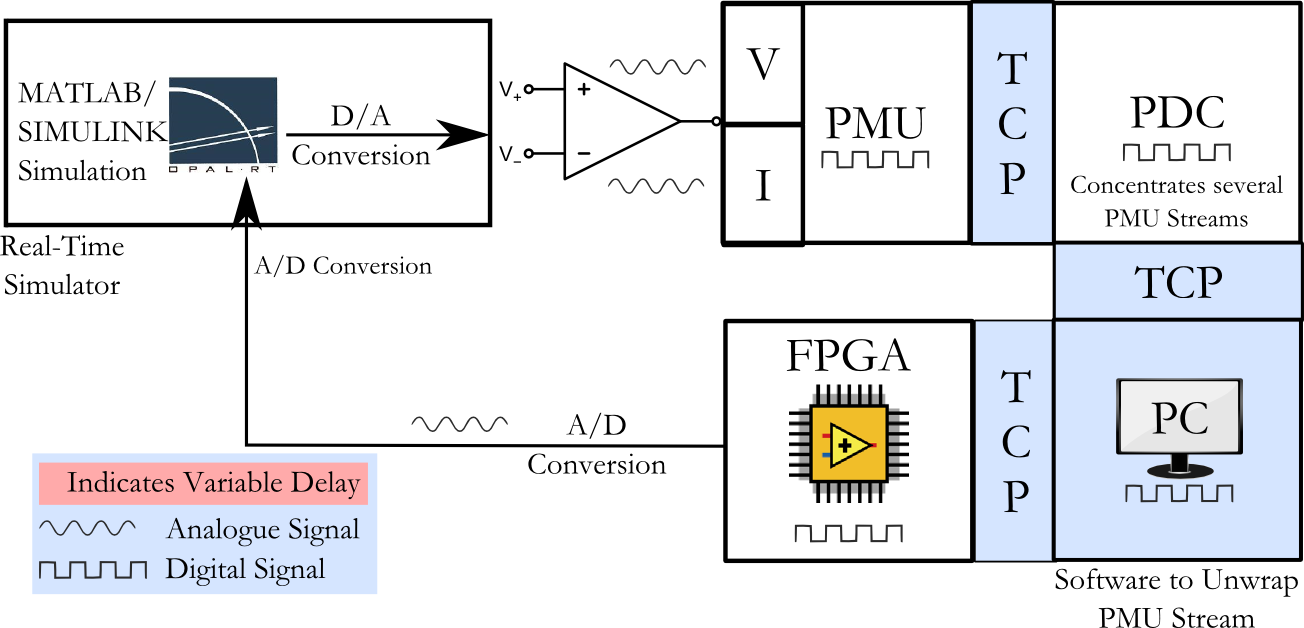
\includegraphics[width=5in]{DataFlow.png}
\caption{General Outline for data flow with digital and analogue components indicated}
\label{Data_path}
\end{figure*}

\subsection{Motivation}
The growth of power system interconnections between previously unconnected areas has given rise to the phenomenon of inter-area oscillations. These are low frequency (0.1-2 Hz.) oscillations where the generators of one synchronous area oscillate against those of another area. Damping for these oscillations is generally poor and if they are allowed to grow, they can lead to disconnection of the ties or a collapse of the power system. A famous example of the latter was the August 1996 blackout of the WSCC system in the USA \cite{NAERC}. Although the purpose of system interconnection was to increase stability, the present situation of the power system incorporates renewable energy sources and power trading corridors, both of which impact system stability.\\

\subsection{Previous Experiences}
Modern solutions to this problem involve using Power System Stabilisers (PSS) with locally available signals. These are effective at damping intra-area modes with good observability but may not be as effective at damping inter-area modes \cite{Dmello} \cite{localREMcomparison}. A theoretical analysis of the advantages of using wide-area signals as a damping input is presented in \cite{Yuwa}. Field-test experiences with WAPOD controllers from Norway and China are presented in \cite{WAPODNorway} and \cite{WAPODChina} respectively.

\subsection{Paper Outline}
This paper is organised as follows.

Section \ref{background} outlines the hardware and software components used together with an overview of the Phasor POD algorithm.

Section \ref{arch} examines the details of the architecture developed for this controller and the various stages of refinement and changes made to it. Section \ref{HILtest} presents the results of the Hardware-in-the-loop tests performed and conclusions are drawn in Section \ref{conclusion}.

\section{Background}\label{background}

\subsection{Phasor POD Algorithm}
The Phaso-POD algorithm was developed by \"{A}ngquist and Gama\cite{PhasorPOD} and forms the core of this work. The algorithm was selected due to its wide applicability and the fact that it does not depend on network topology. Typical model-linearisation based damping algorithms rely on intensive calculations and are typically valid for a particular network operating point. The Phasor-POD algorithm only requires knowledge of the inter-area oscillation frequency, which is generally known from system studies or can be determined from synchrophasor measurements. In the two-area network used here, the inter-area oscillation frequency is known to be 0.64Hz. Consider Equation \ref{PODEqn} which is a representation of a general signal $s(t)$, as an average valued component and an oscillating component.\\

\begin{equation}
%\begin{multlined}
s(t)={s}_{avg}+\mathrm{Re}\left\{{\stackrel{\to }{s}}_{ph}\cdot {e}^{{j}^{wt}}\right\}
%\mbox{where, } {\stackrel{\to }{s}}_{ph} \mbox{ is a complex phasor, rotating at the frequency }\\ \omega
\label{PODEqn}
%\end{multlined}
\end{equation}

$\stackrel{\to }{s}_{ph}$ is a complex phasor, rotating at the frequency $\omega$ \cite{PhasorPOD}. The Phasor-POD algorithm uses the known oscillation frequency to set up a co-orindate system rotating at this frequency and continuously extracts a phasor representing the magnitude of oscillation\cite{PhasorPOD}. This extracted signal can subsequently be used as a modulating input to a controllable device such as a FACTS device or a generator's AVR system. The implementation of the algorithm used here is based on Almas and Vanfretti's Simulink implementation \cite{PhasorPODImplement} and uses three inputs : the search frequency, $\omega_{cs1}$, the sampling time $T_{s}$, the phase correction $alpha$ in addition to a signal scaling factor.\\

\subsection{Hardware and Software Used}
\subsubsection*{Real-Time Controller} The real-time implementation of the Phasor-POD algorithm in this work is based on the Compact Reconfigurable Input Output (cRIO) from National Instruments. The cRIO 9081 \cite{cRIO9081} is used for the implementation of the algorithm. It has an onboard Field Programmable Gate Array (FPGA) in addition to a 1.06 GHz. Intel Celeron processor for real-time control applications\cite{cRIO9081}.\\

\subsubsection*{Phasor Measurement Units}
The inputs to the real-time controller would come from a C37.118-compliant synchrophasor data stream. Measurement data for this stream would be generated by two PMU's which monitor three-phase currents and voltages at different points on the power network. In this work, two cRIO9076 real-time controllers \cite{cRIO9076} were deployed as PMU's.\\

\subsubsection*{Real-Time Simulator}
The e\textsc{megasim} real-time simulator from OPAL RT \cite{eMEGASIM} was used for simulating the two-area network in real-time. This simulator allowed for hardware-in-the-loop tests to be carried out using its analogue input and output terminals. Voltage and current signals were extracted from the simulator's analogue outputs and fed to analogue amplifiers. These amplified signals were then wired to the current and voltage inputs of PMU's. Similarly, the damping signal generated by the Phasor-POD algorithm was then wired back to the simulator's analogue input terminals for use in the simulation. Figure \ref{Data_path} presents the entire signal path including the external, closed-loop control.\\

\subsubsection*{Software}
The test-case network model used here was based on a \textsc{Simulink} demo available with SimPowerSystems. This was modified to include an average-valued SVC model, identical to that used in \cite{PhasorPODImplement}. The \textsc{Simulink} model was modified and prepared for real-time simulation. Software code for the cRIO was written using LabView's Real-Time modules. OPAL RT's e\textsc{megasim} platform uses \textsc{Matlab} code and \textsc{Simulink} models. Software development was done on a workstation computer. Code was loaded on the various devices (cRIO contollers, RT Simulator) over a TCP network.\\

\begin{figure}[!t]
\centering
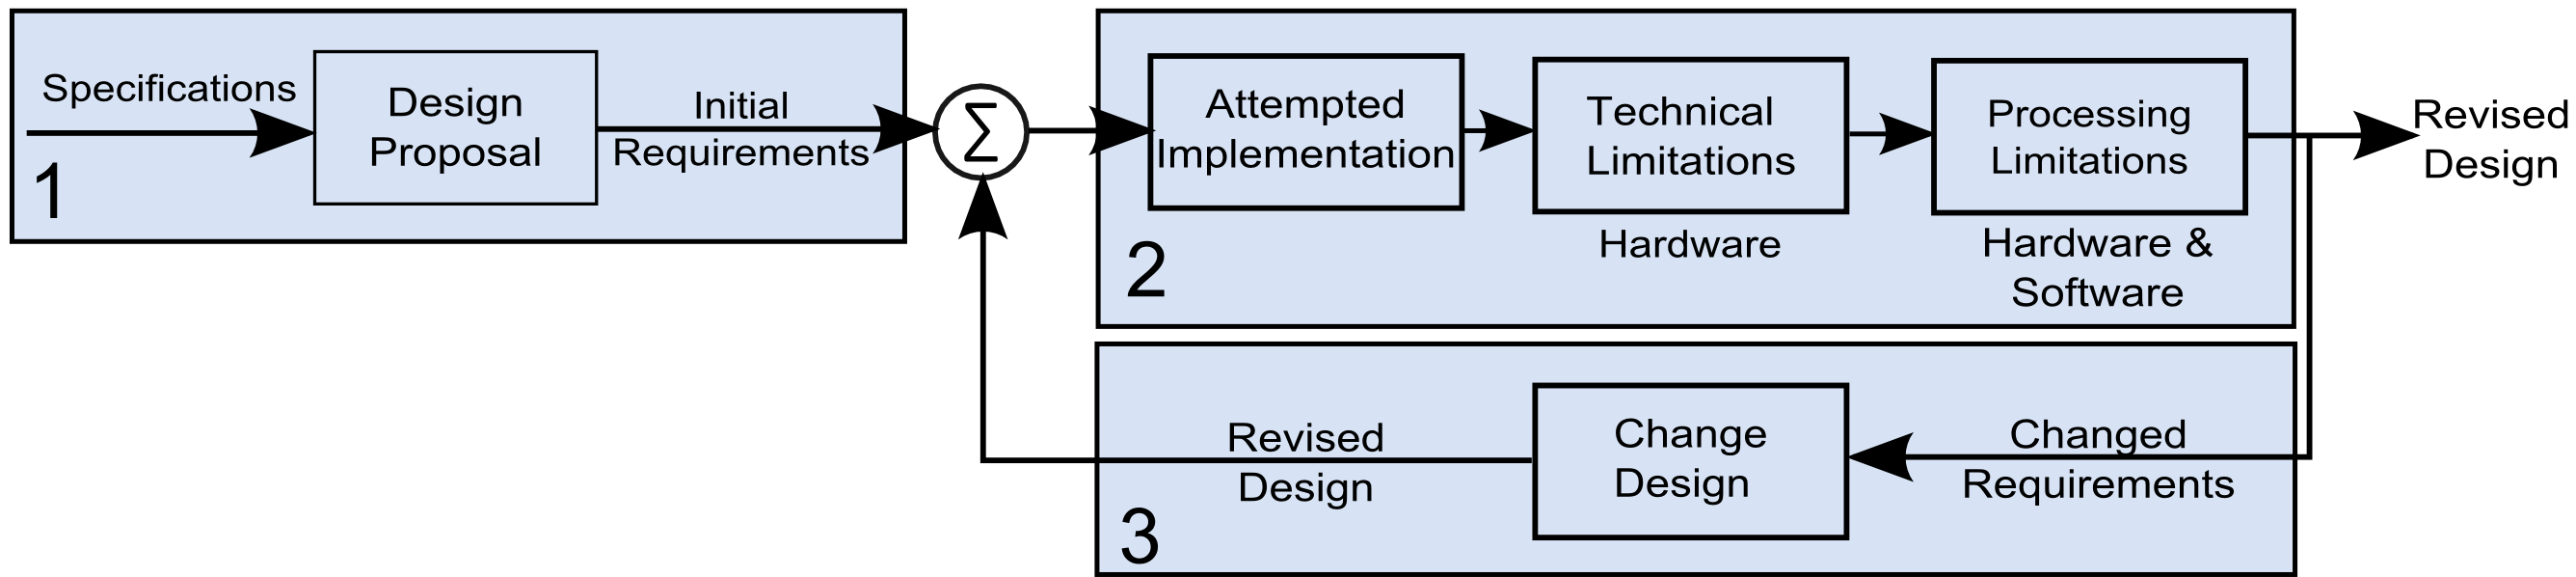
\includegraphics[width=3.5in]{RevisionFlow.png} 
\caption{Iterative Revision Flow Diagram}
\label{fig:RevisionFlow}
\end{figure}

\section{Architecture Development Process}\label{arch}

Before beginning the development process, a software development methodology was adopted with the aim of streamlining the process. \textbf{(Why this method and not others??)} The approach followed here is based on the Waterfall method detailed in \cite{WaterfallCoding}. The approach broadly includes the four steps from \cite{WaterfallCoding} viz. 

\begin{enumerate}
\item Initial Investigation
\item Requirements Definition
\item Architecture Design
\item Coding and Implementation
\end{enumerate}

The linear waterfall method was modified to be iterative so as to account for various constraints and to also account for revisions in the initial definition caused by these constraints. This iterative process is illustrated in Figure \ref{fig:RevisionFlow}.

Several reasons were behind the choice of an iterative design approach. Chief among them was the cRIO hardware itself. As an implementation on this hardware had not been attempted earlier, the limitations of the hardware were unknown. Based on the limitations faced during an implementation attempt, the design and features incorporated would be revised to fit within the limitations of the hardware. \\

\begin{figure}[!t]
\centering
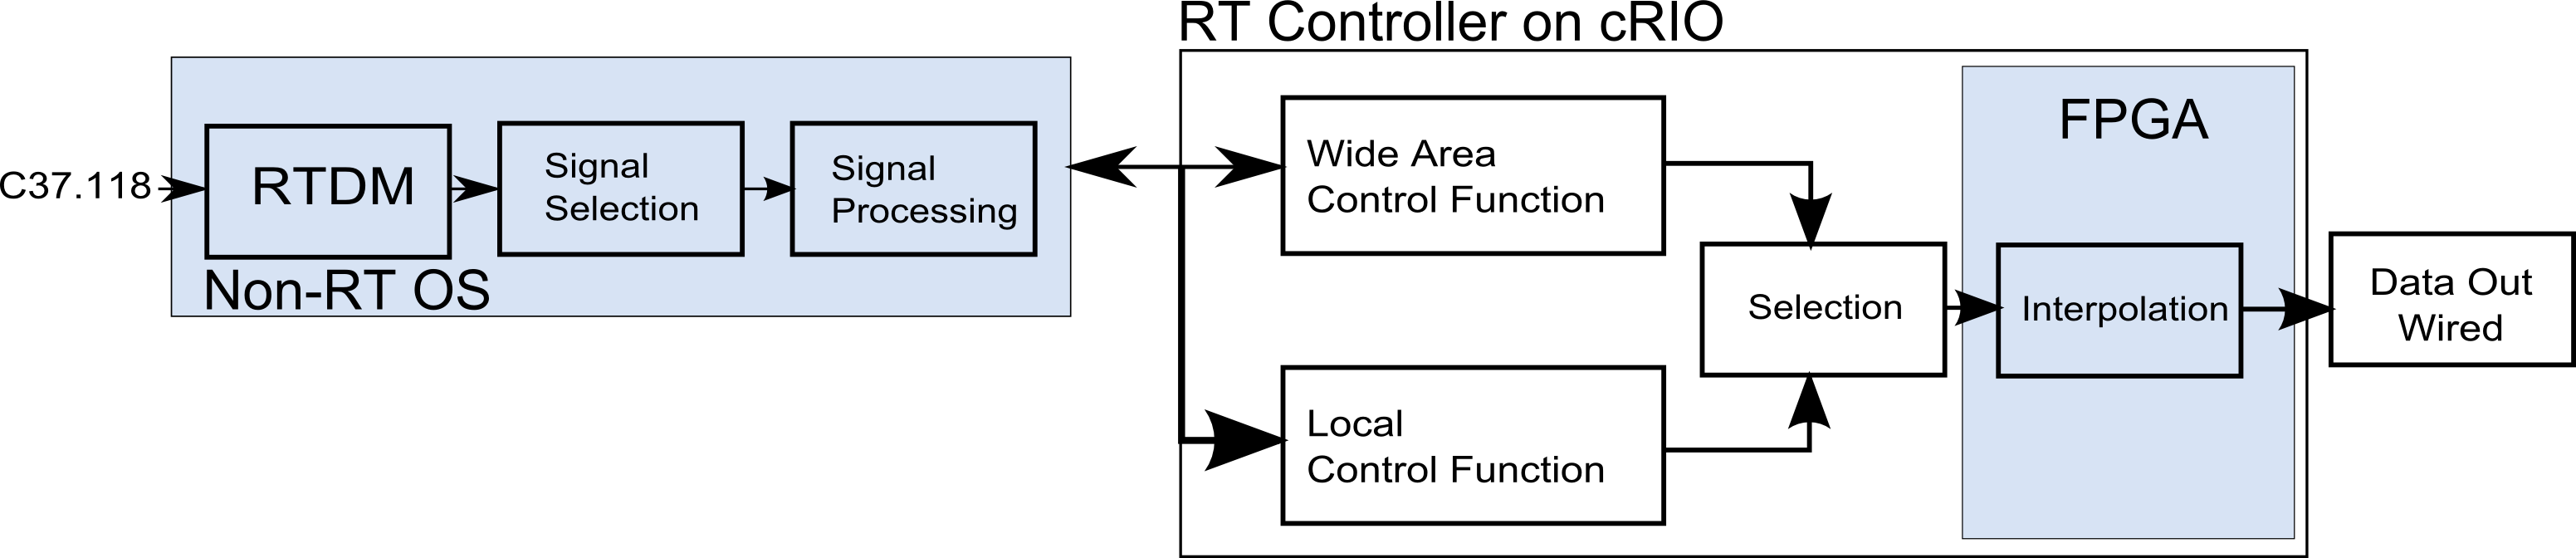
\includegraphics[width=3.5in]{Revision.png} 
\caption{Iterative Revision Flow Diagram}
\label{Revision1}
\end{figure}

\subsection{Constraints}

Before defining requirements at each stage of the software implementation, the possible constraints at each stage of the test set-up were considered. The test set-up shown in Figure \ref{Data_path} is used to illustrate the constraints faced.

\subsubsection*{Differing Loop Rates}
The power system simulation running on the real-time simulator was run at a loop rate of 50$\mu$s. This meant that the simulator would generate new values for currents and voltages every 50$\mu$s. and would also expect data from the HIL system every 50$\mu$s. The constraint here was the data reporting rate of the PMU's used which was a maximum of 50 samples per second or one sample every 20ms. This was much slower that the 50$\mu$s. loop rate of the real-time simulator. A solution would be required for this.

\subsubsection*{FPGA Accuracy}
While the exact role of the FPGA in this implementation was not known in advance, it brought with it some limitations. Chief among these was the limitation on data accuracy due to the f fact that all calculations together with circuit logic would be implemented in hardware.

\section{Architecture Implementation and Refinement}

Figure \ref{fig:RevisionFlow} shows the three stage design process with design proposal, implementation and revision. To begin with, only the controller specifications were available. These were used to draft a design proposal. An implementation attempt was made using this draft proposal. When the additional limits imposed by the software and hardware platforms were included, some goals of the original code would have to revised. With these limitations, the original design was modified to generate a revised design. An attempt was then made to implement this revised design. If further limitations were encountered, the design was further modified. This iterative process was repeated till a working implementation was reached.\\

\subsubsection{Initial Design}

Initially, the goal was to keep the controller (the cRIO) independent of any other devices. Such a controller would be able to receive synchrophasor data (in the C37.118 format) directly over the communication network (ethernet) and extract measurement data. The architecture block diagram is shown in Figure  \ref{fig:InitialArch}. This controller was completely autonomous, with automated signal selection and processing. This design would be able to compute observability indices for the different input signals and then automatically select the one with the highest observability of a particular mode. This design also incorporated two control functions, a wide area control function and a local control function. The wide area control function selected for implementation was the phasor-based oscillation damping control algorithm\cite{PhasorPOD}. The local control function would use locally available data and implement the control function in a manner similar to a Power System Stabiliser (PSS). Automatic switching between the two functions was also considered. If the signal to noise ratio in the wide area signal deteriorated or if the signal delay became prohibitively high, the controller would switch to the local signal or a back-up wide area signal automatically. The principal consideration in this design was the limited resources available on the FPGA and the complexity of the algorithms to be implemented. This required implementation of all algorithms and computation sections on the RT section of the cRIO. In addition, the RT controller chosen has tremendous flexibility as algorithms are implemented using software, rather than hardware as on the FPGA. The RT controller also has more storage space available to implement algorithms. The trade-off was computation speed.\\

\begin{figure}[!th]
\centering
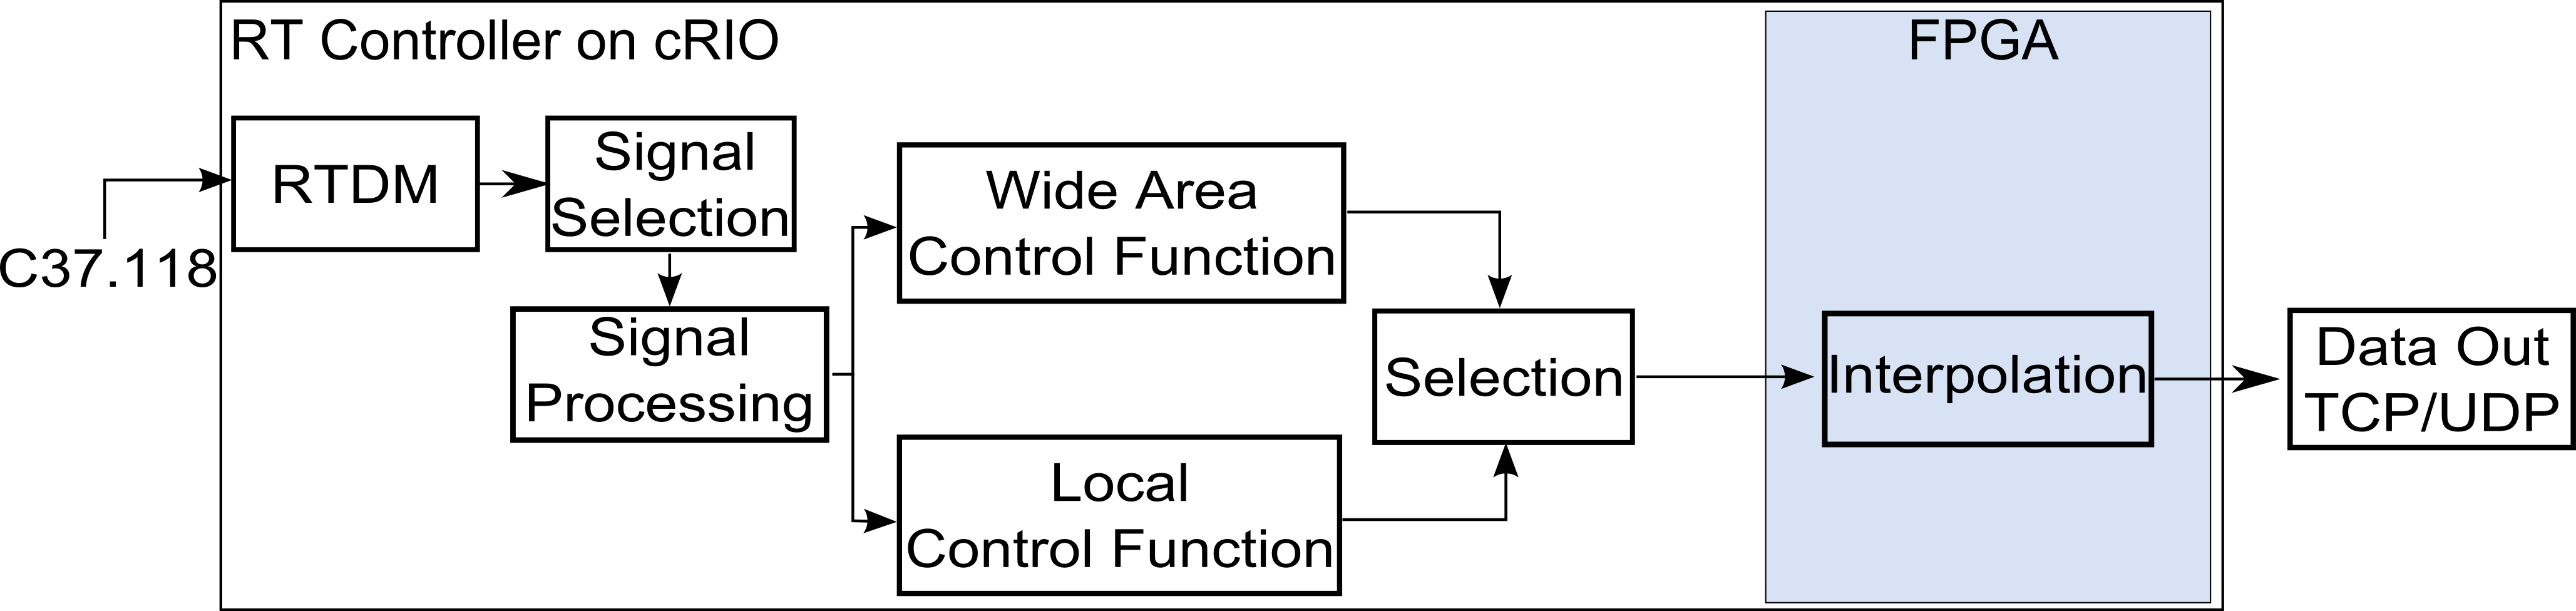
\includegraphics[width=3.5in]{InitialArch}
\caption{Initial Software Architecture}
\label{fig:InitialArch}
\end{figure}


%\begin{figure}[!b]
%\centering
%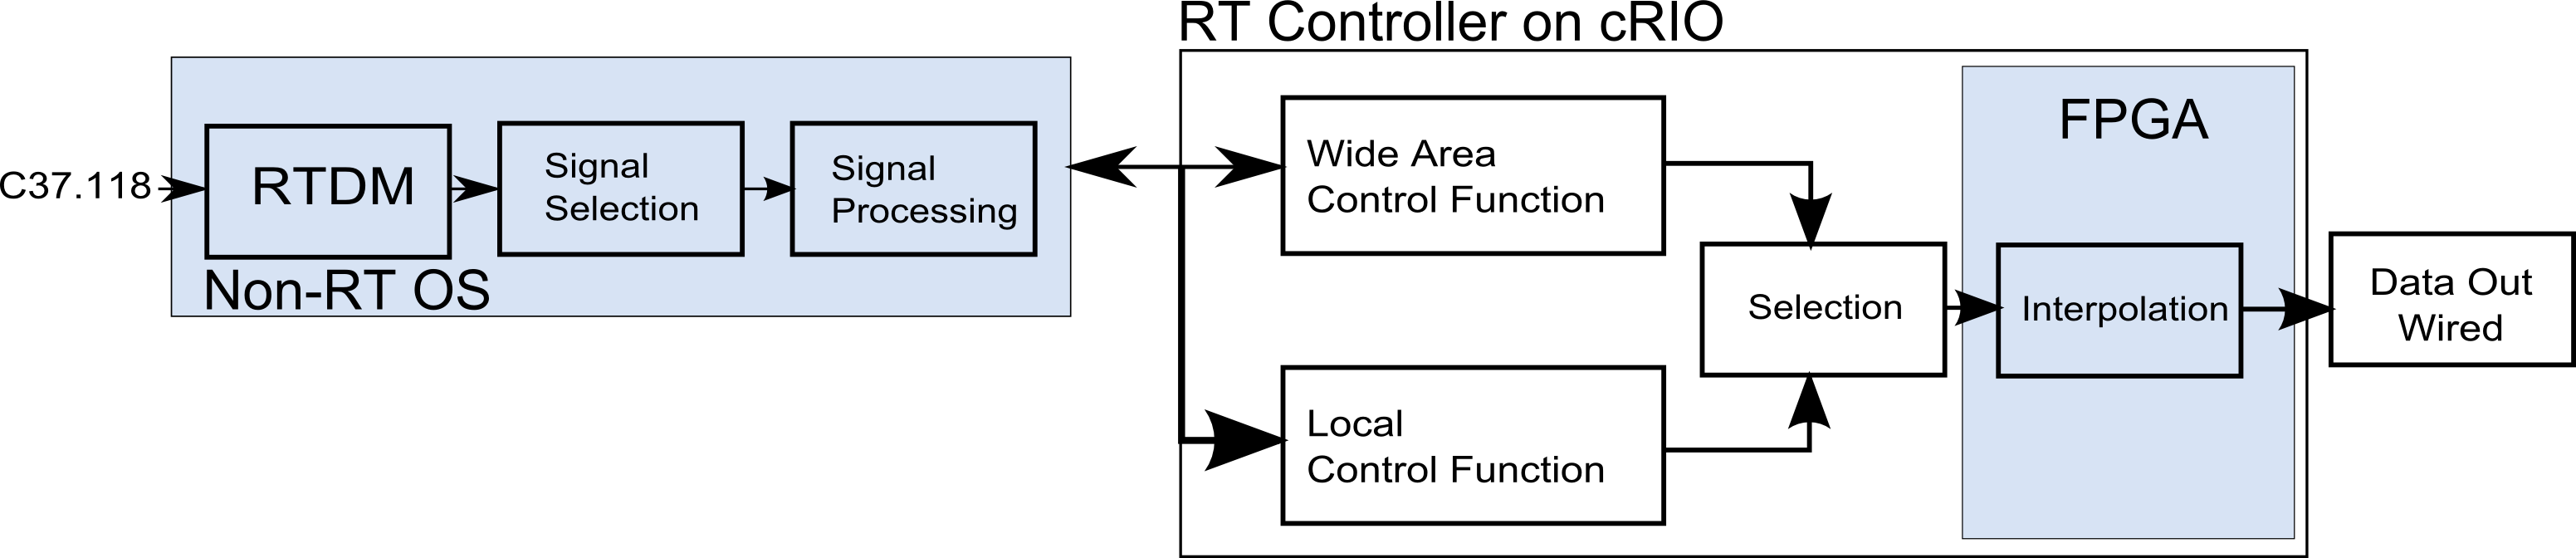
\includegraphics[width=3.5in]{Revision.png} 
%\caption{Iterative Revision Flow Diagram}
%\label{Revision1}
%\end{figure}

This design was faced with a problem of differing loop rates. The real-time simulator runs at a 50$\mu$s time step. The RT controller on the cRIO is not capable of matching this speed. The fastest that it could run was 1ms. Data would thus be generated faster than the RT controller was able to process. The second problem was producing control output at the rate expected by the real-time simulator. The speed constraint of the RT controller meant that it would not be possible to use it (the RT controller) to generate this control signal. To address this issue, this architecture envisaged using the FPGA to perform interpolation between successive data points. The FPGA would run at a loop rate of 50 microseconds, to match the real-time simulator. The region between successive data points would be interpolated using a suitable interpolation algorithm. Data generated by the FPGA would be sent over the communication network back to the real-time simulator for use in the simulation.\\

This design was changed due to limitations of different components. One, no software was available to receive a synchrophasor stream and extract measurement data on the RT controller. This process had to be performed on a desktop computer running a real-time data mediator \cite{SDK} and LabVIEW. Once measurement data from the synchrophasor stream was available, it could be streamed to the real-time controller over the TCP/IP network.\\

Two, data generated by the FPGA could not be sent to the real-time simulator directly over the communication network. Though theoretically possible using a FIFO\footnote{First In First Out} buffer, further work is required. Also, for each succesive data point received by the real-time controller, the FPGA would generate 400, interpolated data points. Synchronising the process of generating the control signal and using the generated data on the real-time simulator will be a complex task.\\

Three, the process of data interpolation on the FPGA is complex. To achieve results better than with a simple linear interpolation, a history of past data points is required. This process is in itself complex and also introduces further delay. However, it is simpler than implementing the damping control algorithm on the FPGA. At this stage, FPGA limitations were the principal factor behind chosing to implement the Phasor-POD algorithm on the RT controller.\\

Four, an algorithm for automated signal selection based on observability indices had not been developed. In principle, this too, is possible and can be implemented on the real-time controller in the future when such an algorithm is developed and verified to work. The Phasor POD algorithm input paramaters also change depending on the input used. An approach to determine these parameters iteratively or calculate them from input data is required. This only adds to the complexity.\\

\subsubsection{Development and Revision}

\begin{figure}[!t]
\centering
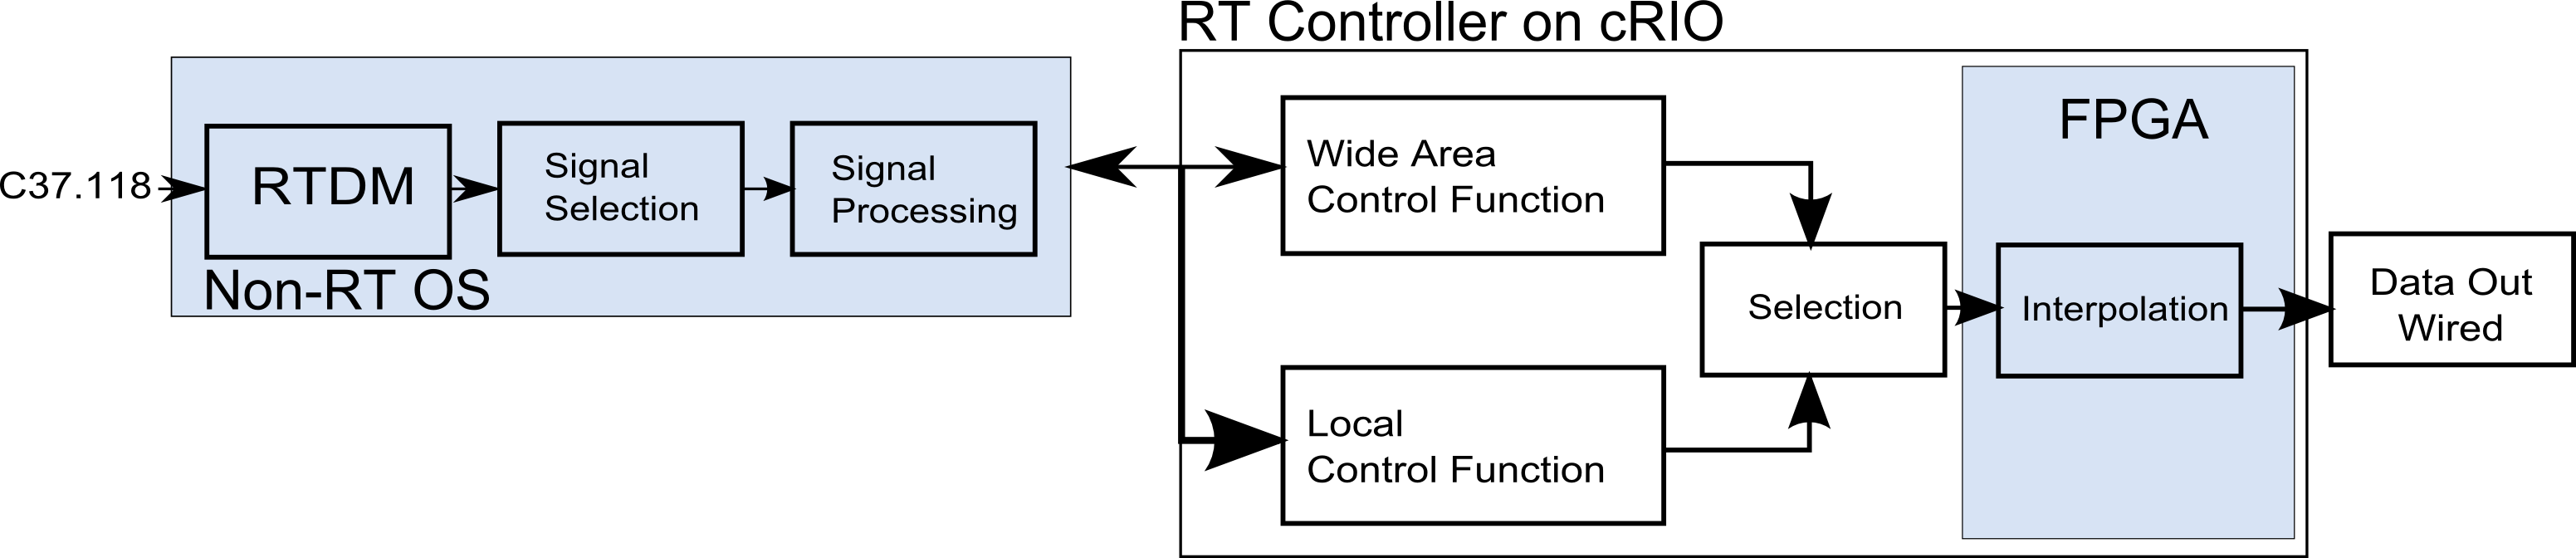
\includegraphics[width=3.5in]{Revision.png}
\caption{Revised Architecture}
\label{fig:Revision}
\end{figure}

With the limitations of the initial architecture in mind, it was revised. In this architecture, the process of  extracting data from the synchrophasor stream was shifted to a workstation computer. The process of signal selection and signal processing was also moved to this computer. Once data was available, it would be sent to the RT controller, over a communication network. The damping control was kept on the RT controller with the FPGA performing the interpolation required to match the read-interval of the real-time simulator. Besides the damping control algorithm, a local control function was maintained on the RT controller. This revision is shown in Figure \ref{fig:Revision}.\\

Here, the complexity of implementing an interpolation algorithm on the FPGA was examined in detail. An implementation was also attempted. It was determined that a simple linear interpolation algorithm would not be sufficiently accurate. Further, the FPGA output was limited by the speed of the RT controller as new data would only be available after a minimum of 1ms at the least (if the RT controller were to run at its maximum speed). \\

An implementation of the damping control algorithm on the RT controller was also tested. The fastest execution speed that could be achieved was in excess of 25ms. This was slower than the reporting rate of the PMUs.\\

Communication between the cRIO and the RT simulator using TCP/IP was also abandoned. Output values of the FPGA were instead hardwired to the real-time simulator's analogue inputs.\\

\subsubsection{Final Implementation}

%\begin{figure}[htb]
%\centering
%\includegraphics[width=1\linewidth]{./Final}
%\caption{Final Software Architecture as Implemented}
%\label{fig:Final}
%\end{figure}

\begin{figure*}[!b]
\centering
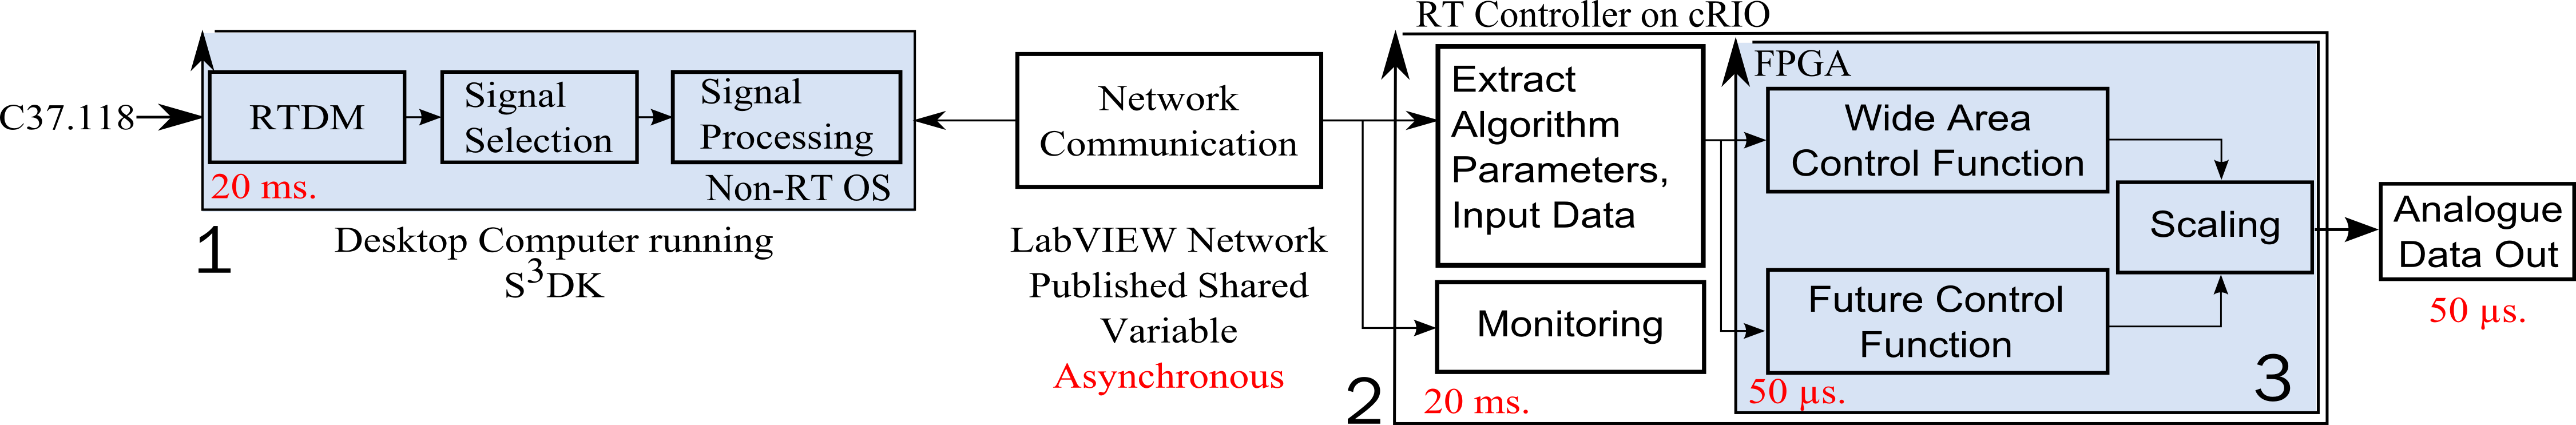
\includegraphics[width=5in]{Final_RT_Arch.png} 
\caption{Final Controller Architecture as Implemented}
\label{Final_arch}
\end{figure*}

At this stage, the damping control algorithm was moved to the FPGA with the RT controller being used only for network communication and data monitoring. The RT controller would only perform the task of receiving measurement data continuously over the network. Phasor POD algorithm parameters and monitoring data would be sent periodically. The local control function was also discarded as it was found to reduce the response speed of the RT controller. If needed and if space permits, the local control function can be implemented on the FPGA. The FPGA is suited to tasks that are repetitive in nature as it has a fast and predictable response time. The desired 50$\mu$s. data output rate could also be maintained as the FPGA was capable of response times of this order. The problem of differing data and loop rates was solved by implementing a basic sample-and-hold algorithm on the FPGA. Data would still be received from the RT controller every 20 ms. but the output would be held constant till the next data point was received and processed. With the Phasor POD algorithm implemented on the FPGA, resource utilization stood at 78\%. Space was still available if further functions need to be implemented on the FPGA. As with the previous design, the process of extracting data from the synchrophasor stream was done on a workstation computer. Signal selection and processing was also done on this computer. This (Figure \ref{Final_arch}) was the final architecture as implemented. Details of the FPGA code as implemented are shown in Figure \ref{FPGA_Blocks}.\\

\begin{figure}[!t]
\centering
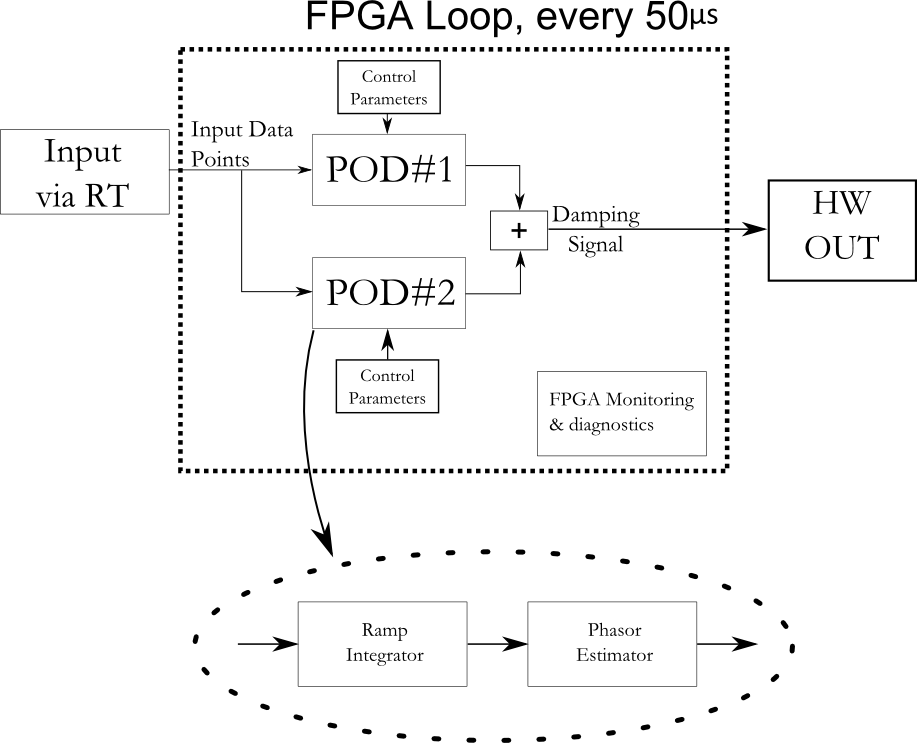
\includegraphics[width=3in]{FPGAOnly.png} 
\caption{Architecture Refinement Schematic}
\label{FPGA_Blocks}
\end{figure}


\section{Hardware-in-the-Loop Test} \label{HILtest}

A setup identical to that outlined in Figure \ref{Data_path} was constructed and used to verify the working of the real-time implementation of the Phasor-POD algorithm. The Phasor-POD algorithm had previously been tested with the two area system. It was verified to be able to keep the system in steady state stability and to restore the system to stability after the application of a minor disturbance. The benchmark for the real-time implementation of the algorithm is thus established.\\

The single-line-diagram of the two-area test network used is shown in Figure \ref{Two_area}. The PMU locations are not shown. The signal generated from the real-time Phasor POD implementation is reinserted in the model at the control system of the SVC. This model was simulated in real-time\\

\begin{figure}[!t]
\centering
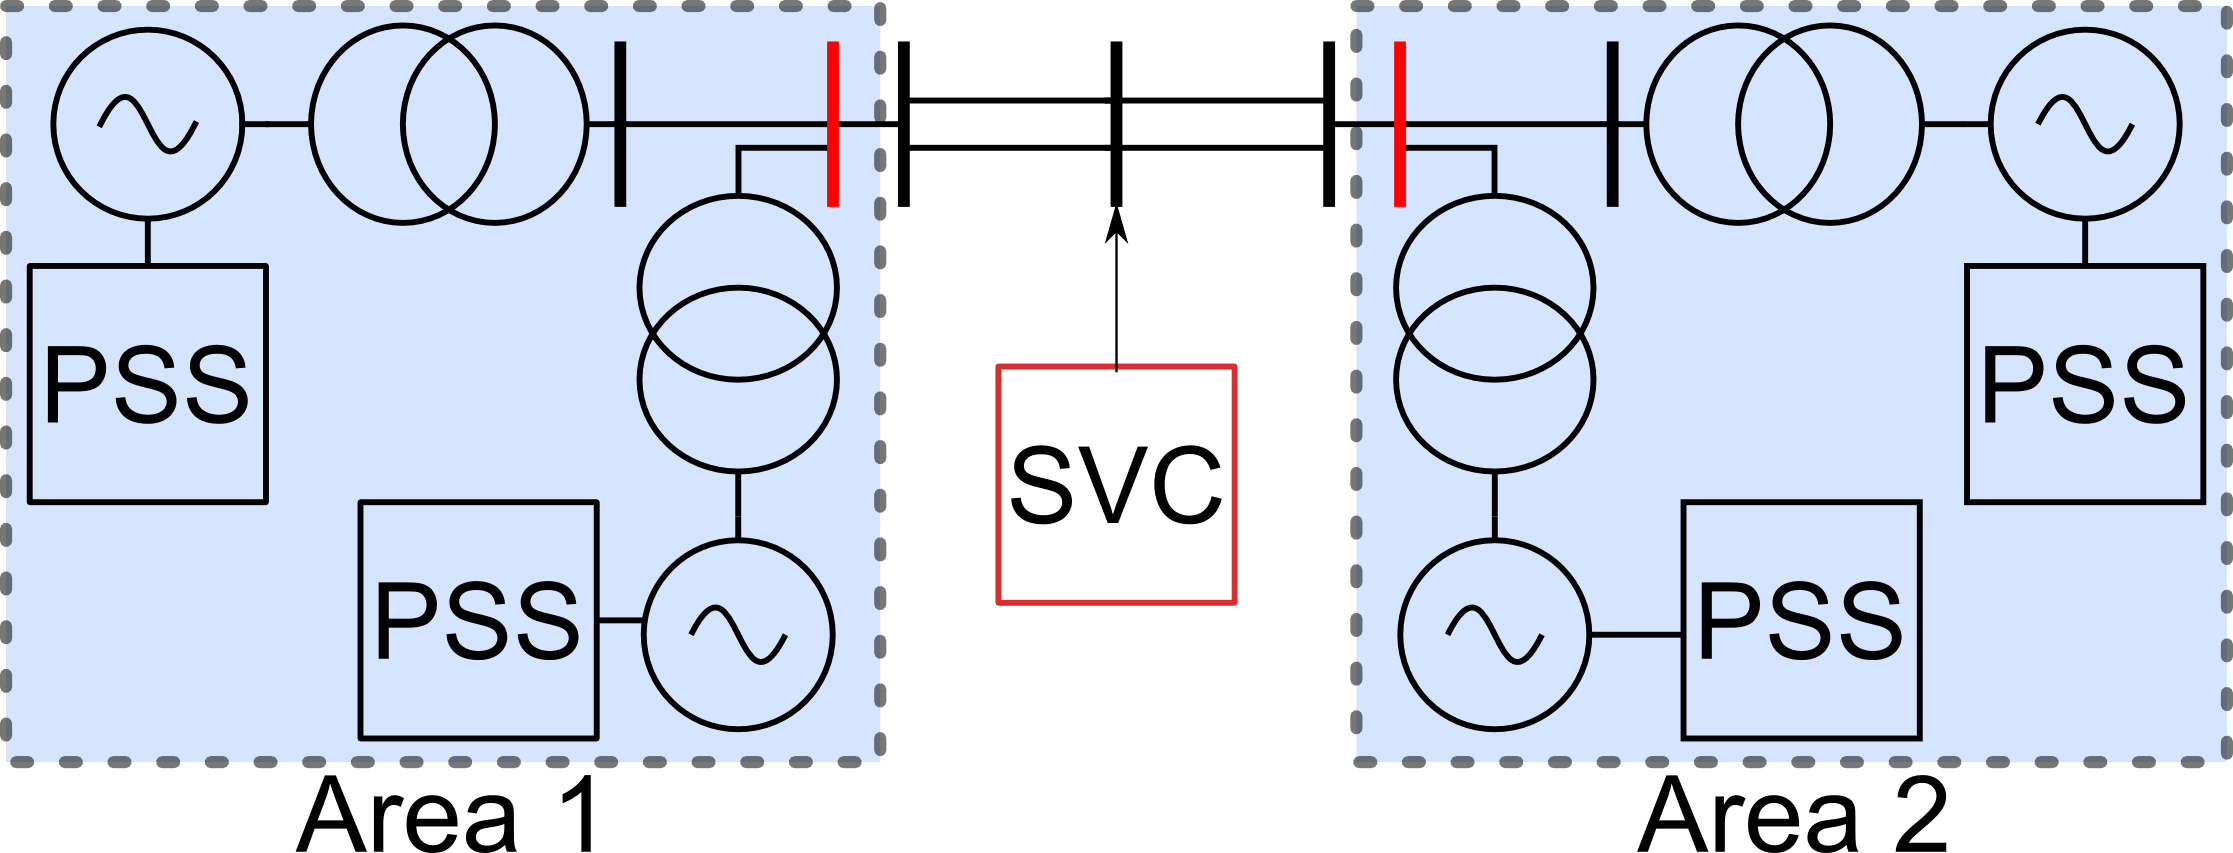
\includegraphics[width=3.5in]{TwoArea.png} 
\caption{Two Area Test network used. PMU measurements are taken from the buses indicated in red.}
\label{Two_area}
\end{figure}

The hardware implementation of the POD algorithm was verified to be able to keep the system stable in steady state. It was also tested with small perturbations applied at one generator to excite the inter-area mode and was verified to work satisfactorily. Figure \ref{Results} shows the performance of the controller with active power used as an input to the Phasor POD algorithm. Though this performance is not identical to similar simulations, it indicated that the real-time implementation of the algorithm was successful.

\begin{figure}[!t]
\centering
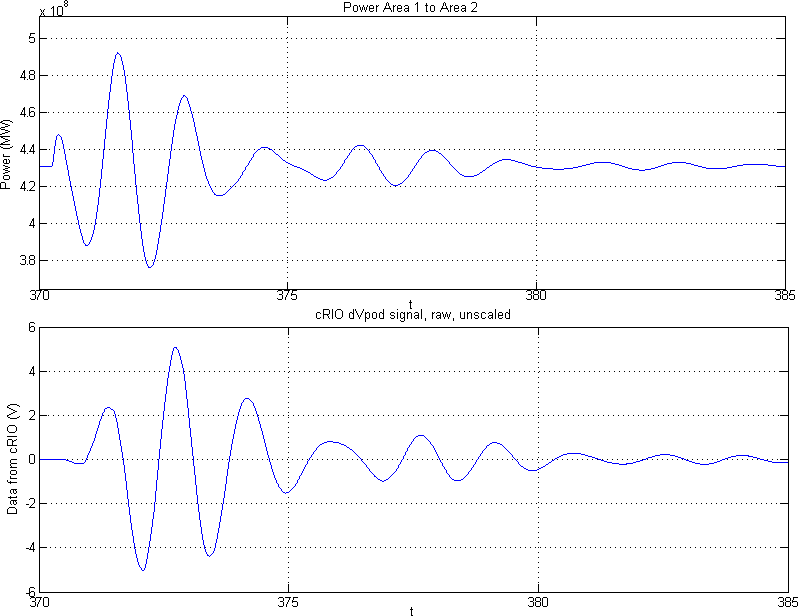
\includegraphics[width=3.5in]{Results.png} 
\caption{Performance of Hardware controller with small disturbance. Active Power magnitude is used as a damping input.}
\label{Results}
\end{figure}

\section{Conclusion} \label{conclusion}
A hardware prototype of a real-time power oscillation damping control system was developed and tested. The developed prototype uses a real-time implementation of the Phasor-POD algorithm. Issues and challenges faced in this implementation are documented and examined. The architecture development \& refinement process for this implementation is also examined in detail. The success of the tests performed indicates that PMU-based wide area controllers have potential applications in power system control and monitoring.



% conference papers do not normally have an appendix


% use section* for acknowledgement
\section*{Acknowledgment}


M.S. Almas is supported by the STRON$g^{2}$rid project, funded by Nordic Energy Research.\\
L. Vanfretti is supported in part by the STRON$g^{2}$rid project, funded by Nordic Energy Research, in part by the STandUP for Energy collaboration initiative and also by the KTH School of Electrical Engineering.\\
The generosity of Schweitzer Engineering Laboratories, Pullman, WA, USA for their donation of protection relays and Megger/Programma, T\"{a}by, Sweden for their donation of numerous pieces of hardware and their technical support is deeply acknowledged.

% trigger a \newpage just before the given reference
% number - used to balance the columns on the last page
% adjust value as needed - may need to be readjusted if
% the document is modified later
%\IEEEtriggeratref{8}
% The "triggered" command can be changed if desired:
%\IEEEtriggercmd{\enlargethispage{-5in}}

% references section

% can use a bibliography generated by BibTeX as a .bbl file
% BibTeX documentation can be easily obtained at:
% http://www.ctan.org/tex-archive/biblio/bibtex/contrib/doc/
% The IEEEtran BibTeX style support page is at:
% http://www.michaelshell.org/tex/ieeetran/bibtex/
%\bibliographystyle{IEEEtran}
% argument is your BibTeX string definitions and bibliography database(s)
%\bibliography{IEEEabrv,../bib/paper}
%
% <OR> manually copy in the resultant .bbl file
% set second argument of \begin to the number of references
% (used to reserve space for the reference number labels box)
\begin{thebibliography}{1}

\bibitem{NAERC} \emph{North American Electric Reliability Council, "Review of selected 1996 Electric System Disturbances in North America,} August 2002. Available Online:  \url{http://www.nerc.com/pa/rrm/ea/System%20Disturbance%20Reports20DL/1996SystemDisturbance.pdf}

\bibitem{PhasorPOD} 
L.~\"{A}ngquist and C.~Gama  \emph{Damping Algorithm based on Phasor Estimation} in Power Engineering Society Winter Meeting, 2001. IEEE, Volume 3, pp. 1160 - 1165  

\bibitem{KundurTwoArea} 
M.~Klein, J. G.~Rogers and P.~Kundur \emph{A fundamental study of inter-area oscillations in Power Systems} IEEE Trans, PWRS, no. 6, pp. 914-921, 1991.

\bibitem{WAPODNorway} Uhlen, K. and Vanfretti, L. and De Oliveira, M. M. and Leirbukt, AB. and Aarstrand, V. H. and Gjerde, J. O. \emph{Wide-Area Power Oscillation Damper implementation and testing in the Norwegian transmission network} in Power and Energy Society General Meeting, 2012 IEEE pp. 1-7

\bibitem{WAPODChina} Li Peng and Wu Xiaochen and Lu Chao and Shi Jinghai and Hu Jiong and He Jingbo and Zhao Yong and Aidong Xu \emph{Implementation of CSG's Wide-Area Damping Control System: Overview and experience} in Power Systems Conference and Exposition, 2009. PSCE '09. IEEE/PES pp. 1-9

\bibitem{eMEGASIM} \emph{eMEGASIM Power Grid Real-Time Digital HArdware in the Loop Simulator} Available Online at : \url{http://www.opal-rt.com/}

\bibitem{Dmello} F. P.~Dmello, and. \ C.~Concordia
  \emph{Concepts of Synchronous Machine Stability as Affected by Excitation Control} IEEE TRANSACTIONS ON POWER APPARATUS AND SYSTEMS, vol. PAS 88, no. 4, 1969. 
  
\bibitem{localREMcomparison}  M. E.~Aboul-Ela, A. A.~Sallam, J. D.~McCalley and A. A.~Fouad, \emph{Damping Controller Design for Power System Oscillations Using Global Signals}, IEEE trans. on Power Systems, Vol. 11, No. 2, May 1996, pp. 767-773
  
\bibitem{PhasorPODImplement} M.~Shoaib Almas and L.~Vanfretti, \emph{Implementation of Conventional PSS and Phasor Based POD for Power Stabilizing Controls for Real-Time Simulation}, IEEE IES IECON14, 29 Oct-1 Nov, 2014, Dallas, USA.

\bibitem{OPALemegasim} eMEGAsim PowerGrid Real-Time Digital Hardware in the Loop Simulator — Opal RT, [Online]. Available: \url{http://www.opal-rt.com/}

\bibitem{WaterfallCoding} \emph{Selecting a Development Approach}, Centre for Medicare and Medicaid Services, USA, February 17, 2005, Accessed on 01 October 2014 Available Online at \url{http://www.cms.gov/Research-Statistics-Data-and-Systems/CMS-Information-Technology/XLC/Downloads/SelectingDevelopmentApproach.pdf}

\bibitem{Chaudhuri} N.S.~Chaudhuri, R.~Majumder and B~ Chaudhuri \emph{Interaction between conventional and adaptive phasor power oscillation damping controllers} in Power and Energy Society General Meeting, 2010 IEEE Minneapolis, MN, 2012 pp. 1-7

\bibitem{SmarTSLab} L.~Vanfretti.; M.~Chenine; M.S.~Almas; R.~Leelaruji; L.~Angquist; L.~Nordstrom, "\emph{SmarTS Lab — A laboratory for developing applications for WAMPAC Systems}," Power and Energy Society General Meeting, 2012 IEEE , vol., no., pp.1,8, 22-26 July 2012

\bibitem{sVARdamp} E.V~Larsen and E.H~Chow, General Electric Company, NY, \emph{Application of Static VAR Systems for System Dynamic Performance}, 1987 IEEE pp. 43-46

\bibitem{Yuwa}  L.~Vanfretti, Y.~Chompoobutrgool, and J.H.~Chow, \emph{Chapter 10: Inter-Area Mode Analysis for Large Power Systems using Synchrophasor Data}, Book Chapter, in Coherency and Model Reduction of Large Power Systems, Joe H. Chow (Ed.), Springer, 2013. Available Online at \url{http://www.springer.com/energy/systems%2C+storage+and+harvesting/book/978-1-4614-1802-3}

\bibitem{cRIO9081} \emph{Operating Instructions and Specifications Compact RIO NI cRIO-9081/9082}, National Instruments, Available Online at \url{http://www.ni.com/pdf/manuals/375714a.pdf}
  
\bibitem{cRIO9076} \emph{Operating Instructions and Specifications Compact RIO NI cRIO-9075/9076}, National Instruments, Available Online at \url{http://www.ni.com/pdf/manuals/375650b.pdf}

\bibitem{LabviewTemplate} \emph{FPGA Control on Compact RIO Sample Project Documentation}, National Instruments, Available Online at \url{http://www.ni.com/white-paper/14137/en/}

\bibitem{SDK} Vanfretti, Luigi and Aarstrand, Vemund H. and Almas, M. Shoaib and Peri\'c, Vedran S. and Gjerde, Jan O. , \emph{A Software Development Toolkit for Real-Time Synchrophasor Applications},  IEEE PES Grenoble PowerTech, 2013

\bibitem{MATLABexample} I~Kamwa \emph{Performance of Three PSS for Interarea Oscillations} SimPowerSystems Examples, \textsc{Matlab} R2011a

\bibitem{PSSDocumentation} \emph{Generic Power System Stabilizer} Documentation distributed with \textsc{Matlab} R2014a Available online at \url{http://www.mathworks.se/help/physmod/sps/powersys/ref/genericpowersystemstabilizer.html}

\end{thebibliography}




% that's all folks
\end{document}


